\documentclass[12pt,a4paper]{article}

\usepackage[a4paper,text={16.5cm,25.2cm},centering]{geometry}
\usepackage{lmodern}
\usepackage{amssymb,amsmath}
\usepackage{bm}
\usepackage{graphicx}
\usepackage{microtype}
\usepackage{hyperref}
\usepackage{minted}
\setlength{\parindent}{0pt}
\setlength{\parskip}{1.2ex}

\hypersetup
       {   pdfauthor = {  },
           pdftitle={  },
           colorlinks=TRUE,
           linkcolor=black,
           citecolor=blue,
           urlcolor=blue
       }






\begin{document}



\begin{minted}[texcomments = true, mathescape, fontsize=\small, xleftmargin=0.5em]{julia}
using Main.DN3
\end{minted}

\section{Matematično nihalo}
Martin Starič

Kotni odmik $\theta(t)$ (v radianih) pri nedušenem nihanju nitnega nihala opišemo z diferencialno enačbo

\[
\frac{g}{l} sin(\theta(t)) + \theta^{''}(t) = 0, \theta(0) = \theta_0, \theta^{'}(t) = \theta^{'}_0
\]
Kjer je g težni pospešek l pa dolžina nihala. Zgornjo diferencialno enačbo drugega reda je treba spremeniti v diferencialno enačbo prvega reda in sicer

\[
\theta^{\prime}(t) = v(t)
\]
\[
v^{\prime}(t) = -\frac{g}{l} \sin(\theta(t))
\]

Za izračun naslednjega približka $\theta$ in $\theta^{'}$ bomo na DE prve stopnje uporabili Runge-Kutta četrtega reda. 


Uporaba približka odmika na nihalu dolžine 1 ob času 10s, začetnem kotnem odmiku $\frac{\pi}{2}$, kotnem pospešku 0 in n = 1000.


\begin{minted}[texcomments = true, mathescape, fontsize=\small, xleftmargin=0.5em]{julia}
l = 100.0
t = 10.0
theta0 = pi/2
dtheta0 = 0.0
n = 10000
nihalo(l,t,theta0,dtheta0,n)
\end{minted}
\begin{minted}[texcomments = true, mathescape, fontsize=\small, xleftmargin=0.5em, frame = leftline]{text}
-1.4047199227643241
\end{minted}

Sedaj primerjajmo Matematično in Harmonično nihalo s pomočjo grafov časa odvisnosti od energije tako, da imata obe nihali ista začetna pogoja in seveda dolžino.


\begin{minted}[texcomments = true, mathescape, fontsize=\small, xleftmargin=0.5em]{julia}
using Plots
odmiki,hitrosti = veckratno_nihalo(1.0,10.0,1.0,1.0,n)
harmonicniodmiki, harmonicnehitrosti = veckratno_harmonicno_nihalo(1.0,10.0,1.0,1.0,n)
size = range(0,stop = 10.0, length = n+1)
\end{minted}
\begin{minted}[texcomments = true, mathescape, fontsize=\small, xleftmargin=0.5em, frame = leftline]{text}
0.0:0.001:10.0
\end{minted}

Sprva ustvarimo graf časa odvisnosti od odmika.


\begin{minted}[texcomments = true, mathescape, fontsize=\small, xleftmargin=0.5em]{julia}
p = plot(size, odmiki, xlabel="Čas (s)", ylabel="Odmik", title="Matematično in Harmonično nihalo", label="Matematično nihalo")
plot!(p, size, harmonicniodmiki, label="Harmonično nihalo")
\end{minted}
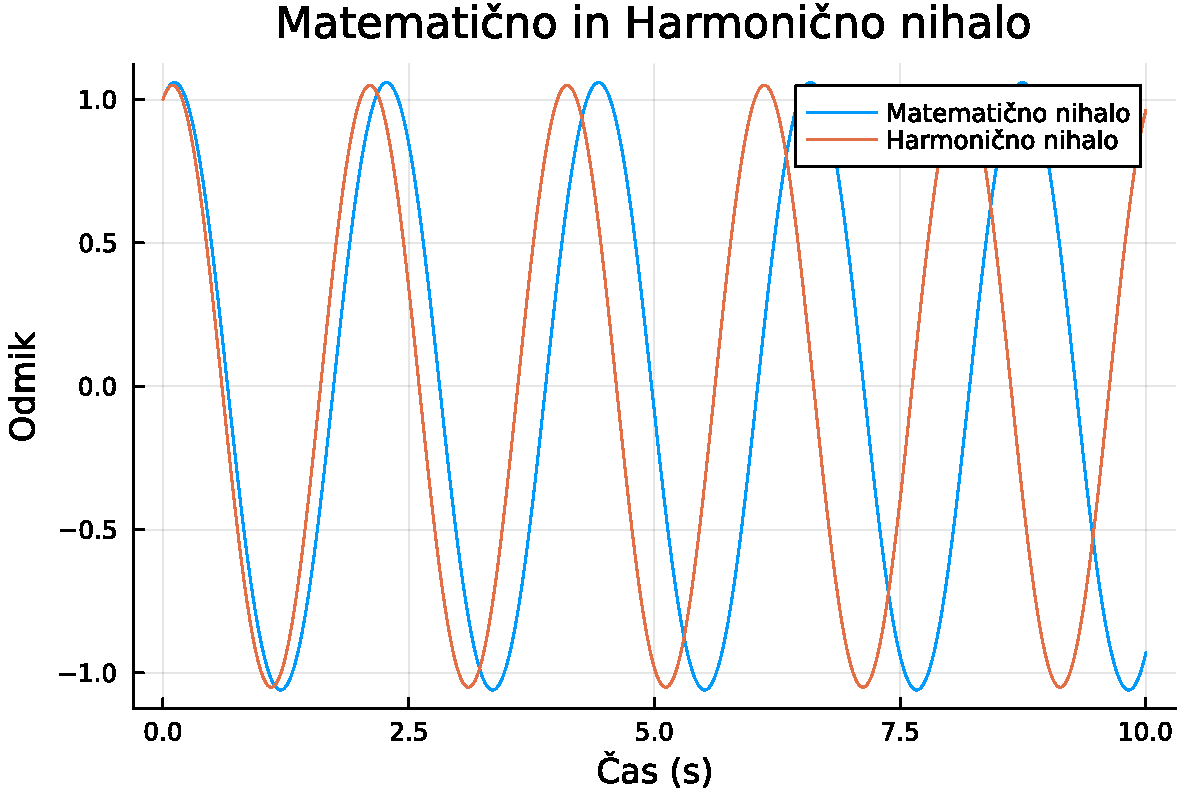
\includegraphics[width=\linewidth]{jl_xzhxDb/demo_4_1.pdf}

Sedaj pa še graf časa odvisnosti od Kinetične energije.


\begin{minted}[texcomments = true, mathescape, fontsize=\small, xleftmargin=0.5em]{julia}
p = plot(size, hitrosti, xlabel="Čas (s)", ylabel="Kinetična energija", title="Matematično in Harmonično nihalo", label="Matematično nihalo")
plot!(p, size, harmonicnehitrosti, label="Harmonično nihalo")
display(p)
\end{minted}
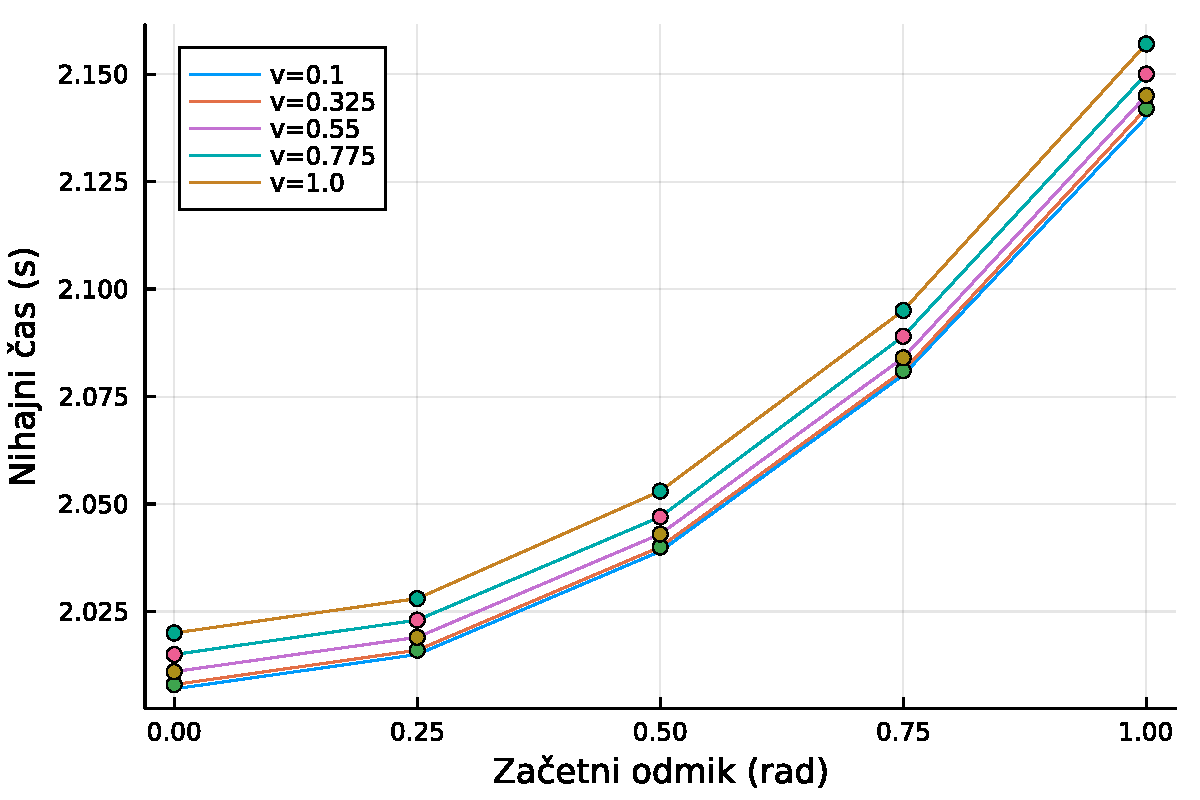
\includegraphics[width=\linewidth]{jl_xzhxDb/demo_5_1.pdf}

Oglejmo si še, kako se nihajni čas spreminja ob različnih začetnih pogojih pri matematičnem nihalu.


\begin{minted}[texcomments = true, mathescape, fontsize=\small, xleftmargin=0.5em]{julia}
zacetni_odmiki = range(0.0, stop=1.0, length=5)
zacetne_hitrosti = range(0.1, stop=1.0, length=5)
casi = zeros(length(zacetni_odmiki), length(zacetne_hitrosti))

for i in 1:length(zacetni_odmiki)
    for j in 1:length(zacetne_hitrosti)
        casi[i,j] = nihajni_cas(1.0,10.0,zacetni_odmiki[i],zacetne_hitrosti[j],n)
    end
end

p = plot(zacetni_odmiki, casi[:, 1], xlabel="Začetni odmik (rad)", ylabel="Nihajni čas (s)", label="v=0.1")
for j in 2:length(zacetne_hitrosti)
    plot!(p, zacetni_odmiki, casi[:, j], label="v=$(zacetne_hitrosti[j])")
    scatter!(p, zacetni_odmiki, casi[:, j], marker=:circle, label="")
end

plot(p, title="Nihajni čas za različne začetne pogoje", legend=:topright)
display(p)
\end{minted}
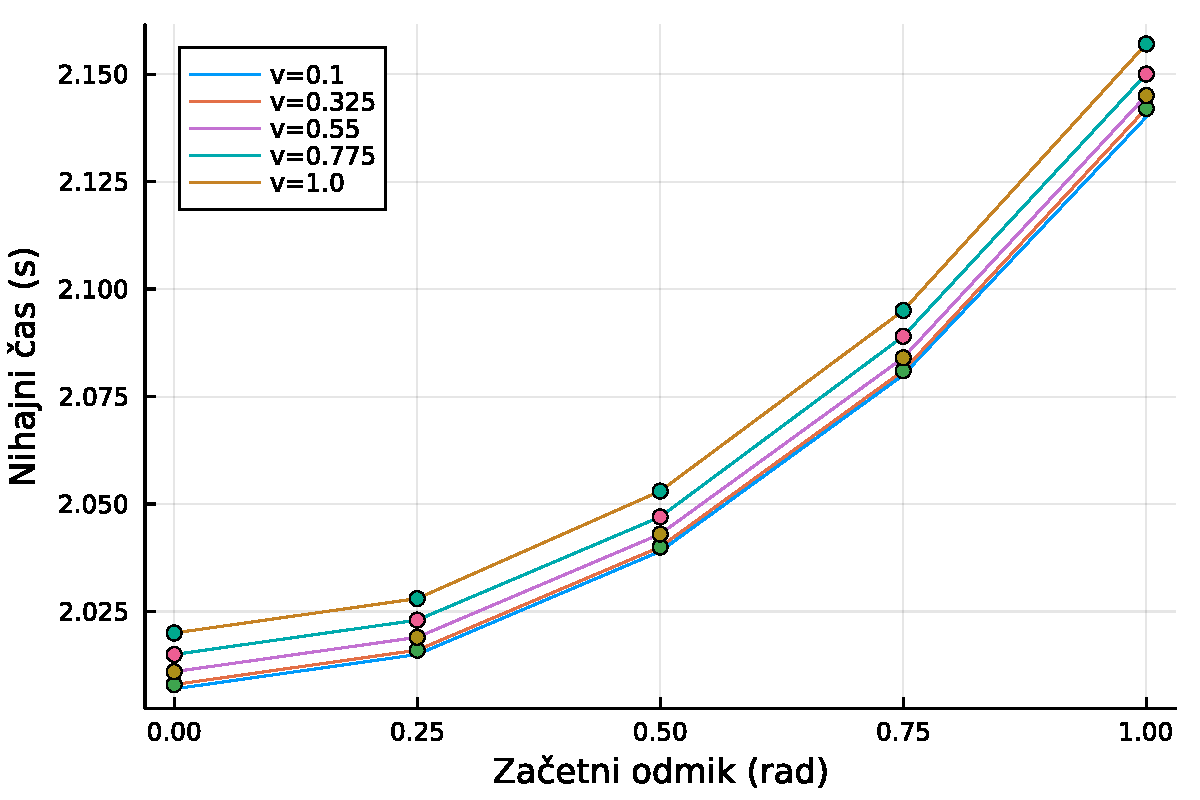
\includegraphics[width=\linewidth]{jl_xzhxDb/demo_5_1.pdf}


\end{document}
